\tikzset{every picture/.style={line width=0.75pt}} %set default line width to 0.75pt        

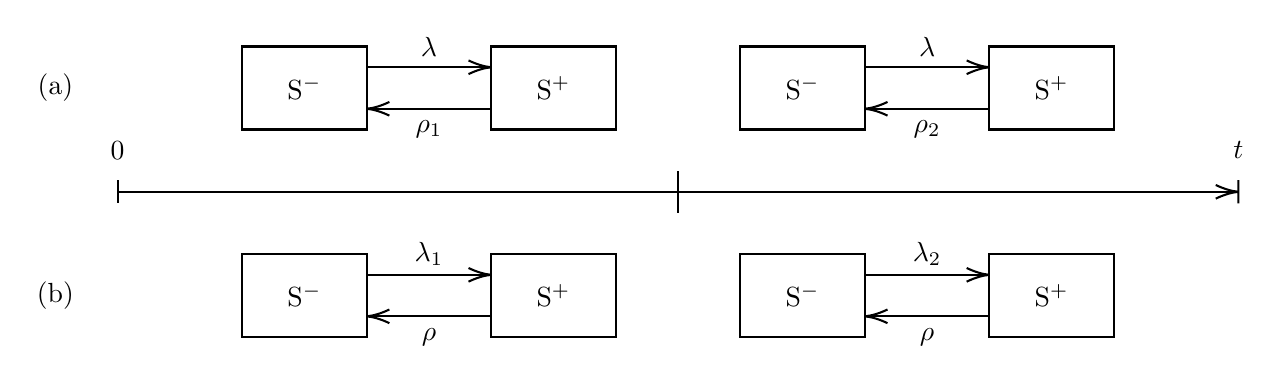
\begin{tikzpicture}[x=0.75pt,y=0.75pt,yscale=-1,xscale=1]
%uncomment if require: \path (0,342.1999969482422); %set diagram left start at 0, and has height of 342.1999969482422

\draw    (240, 100) rectangle (300, 140)   ;
\draw    (360, 100) rectangle (420, 140)   ;
\draw    (300,110) -- (360,110) ;
\draw [shift={(360,110)}, rotate = 180] [color={rgb, 255:red, 0; green, 0; blue, 0 }  ]   (0,0) .. controls (3.31,-0.3) and (6.95,-1.4) .. (10.93,-3.29)(0,0) .. controls (3.31,0.3) and (6.95,1.4) .. (10.93,3.29)   ;

\draw    (360,130) -- (300,130) ;
\draw [shift={(300,130)}, rotate = 360] [color={rgb, 255:red, 0; green, 0; blue, 0 }  ]   (0,0) .. controls (3.31,-0.3) and (6.95,-1.4) .. (10.93,-3.29)(0,0) .. controls (3.31,0.3) and (6.95,1.4) .. (10.93,3.29)   ;

\draw    (480, 100) rectangle (540, 140)   ;
\draw    (600, 100) rectangle (660, 140)   ;
\draw    (600,130) -- (540,130) ;
\draw [shift={(540,130)}, rotate = 360] [color={rgb, 255:red, 0; green, 0; blue, 0 }  ]   (0,0) .. controls (3.31,-0.3) and (6.95,-1.4) .. (10.93,-3.29)(0,0) .. controls (3.31,0.3) and (6.95,1.4) .. (10.93,3.29)   ;

\draw    (540,110) -- (600,110) ;
\draw [shift={(600,110)}, rotate = 180] [color={rgb, 255:red, 0; green, 0; blue, 0 }  ]   (0,0) .. controls (3.31,-0.3) and (6.95,-1.4) .. (10.93,-3.29)(0,0) .. controls (3.31,0.3) and (6.95,1.4) .. (10.93,3.29)   ;

\draw    (180,170) -- (720,170) ;
\draw [shift={(720,170)}, rotate = 180] [color={rgb, 255:red, 0; green, 0; blue, 0 }  ]   (0,5.59) -- (0,-5.59)(0,0) .. controls (3.31,-0.3) and (6.95,-1.4) .. (10.93,-3.29)(0,0) .. controls (3.31,0.3) and (6.95,1.4) .. (10.93,3.29)   ;
\draw [shift={(180,170)}, rotate = 180] [color={rgb, 255:red, 0; green, 0; blue, 0 }  ]   (0,5.59) -- (0,-5.59)   ;
\draw    (240, 200) rectangle (300, 240)   ;
\draw    (360, 200) rectangle (420, 240)   ;
\draw    (480, 200) rectangle (540, 240)   ;
\draw    (600, 200) rectangle (660, 240)   ;
\draw    (300,210) -- (360,210) ;
\draw [shift={(360,210)}, rotate = 180] [color={rgb, 255:red, 0; green, 0; blue, 0 }  ]   (0,0) .. controls (3.31,-0.3) and (6.95,-1.4) .. (10.93,-3.29)(0,0) .. controls (3.31,0.3) and (6.95,1.4) .. (10.93,3.29)   ;

\draw    (360,230) -- (300,230) ;
\draw [shift={(300,230)}, rotate = 360] [color={rgb, 255:red, 0; green, 0; blue, 0 }  ]   (0,0) .. controls (3.31,-0.3) and (6.95,-1.4) .. (10.93,-3.29)(0,0) .. controls (3.31,0.3) and (6.95,1.4) .. (10.93,3.29)   ;

\draw    (600,230) -- (540,230) ;
\draw [shift={(540,230)}, rotate = 360] [color={rgb, 255:red, 0; green, 0; blue, 0 }  ]   (0,0) .. controls (3.31,-0.3) and (6.95,-1.4) .. (10.93,-3.29)(0,0) .. controls (3.31,0.3) and (6.95,1.4) .. (10.93,3.29)   ;

\draw    (540,210) -- (600,210) ;
\draw [shift={(600,210)}, rotate = 180] [color={rgb, 255:red, 0; green, 0; blue, 0 }  ]   (0,0) .. controls (3.31,-0.3) and (6.95,-1.4) .. (10.93,-3.29)(0,0) .. controls (3.31,0.3) and (6.95,1.4) .. (10.93,3.29)   ;

\draw    (450,160) -- (450,180) ;



\draw (390,120) node  [align=left] {S$^{+}$};
\draw (270,120) node  [align=left] {S$^{-}$};
\draw (630,120) node  [align=left] {S$^{+}$};
\draw (510,120) node  [align=left] {S$^{-}$};
\draw (330,100) node  [align=left] {$\lambda $};
\draw (570,100) node  [align=left] {$\lambda $};
\draw (330,140) node  [align=left] {$\rho _{1}$};
\draw (570,140) node  [align=left] {$\rho _{2}$};
\draw (330,200) node  [align=left] {$\lambda _{1}$};
\draw (330,240) node  [align=left] {$\rho $};
\draw (570,240) node  [align=left] {$\rho $};
\draw (570,200) node  [align=left] {$\lambda _{2}$};
\draw (270,220) node  [align=left] {S$^{-}$};
\draw (510,220) node  [align=left] {S$^{-}$};
\draw (390,220) node  [align=left] {S$^{+}$};
\draw (630,220) node  [align=left] {S$^{+}$};
\draw (450,150) node  [align=left] {$\uptau $};
\draw (720,150) node   {$t$};
\draw (180,150) node   {$0$};
\draw (150,120) node  [align=left] {(a)};
\draw (150,220) node  [align=left] {(b)};


\end{tikzpicture}
